% Methodology section
Modeling temporality is central to be able to capture the true essence of complex systems. Components of complex systems interact with one another and evolve across multiple time scales, leading to emergent phenomena that cannot be understood through static or purely structural models. However for modeling such systems, it is sufficient to model the participant components and their interactions as stochastic processes that evolve over time, rather than modeling time explicitly. This implies our model must capture sequences that represent the evolution of states and interactions over time, while preserving causal relationships. The different scales of time are captured by the hierarchical structure of operads, where different levels of the hierarchy can represent dynamics occurring at different time scales, with higher levels operating at slower time scales than lower ones.

We develop a novel mathematical framework, based on WD-operads, to model complex systems through temporal-causal relationships. Our approach enriches the established theory of WD-operads with temporal probability structures, creating operads that naturally capture sequential dynamics and causal interactions.

\subsection{Temporal Probability Spaces}

Let us first define the notion of temporal probability spaces, which will serve as an enriching category for our operads. We denote the category of temporal probability spaces as $\mathbf{TempProb}$.

Each object of $\mathbf{TempProb}$ is a temporal probability space, $\Omega_{\mathcal{W}}$, where each object of the space represents a state of the system at a given time. Hence for each box of the WD-operad $\mathcal{W}$, the space $\Omega_{\mathcal{W}}$ contains the set of all possible execution paths or histories of the system component represented by that box. Additionally, to enable us to assign probabilities to subsets of these execution paths, we equip each temporal probability space with a sigma-algebra $\mathcal{F}$ of measurable events and a probability measure $\mathbb{P}$ that assigns probabilities to these events.

Morphisms in $\mathbf{TempProb}$ are adapted stochastic processes that preserve the temporal structure of the spaces, ensuring that information flows consistently through time. A morphism between two temporal probability spaces represents how the probabilistic evolution of one system component conditions or influences the probability distribution over possible evolutions of another component over time. For example, a morphism $K: \Omega_{\mathcal{W}_1} \to \Omega_{\mathcal{W}_2}$ between two temporal probability spaces can be viewed as a stochastic kernel that maps each execution path in $\Omega_{\mathcal{W}_1}$ to a probability distribution over execution paths in $\Omega_{\mathcal{W}_2}$, while respecting the temporal ordering of events. At time $t$, given history up to time $t$ in $\Omega_{\mathcal{W}_1}$, the morphism $K$ tells us the conditional probability distribution over possible states at time $t$ in $\Omega_{\mathcal{W}_2}$.

Formally, the category $\mathbf{TempProb}$ is defined as follows:

\begin{itemize}
    \item \textbf{Objects}: Temporal probability spaces $(\Omega, \mathcal{F}, \{\mathcal{F}_t\}_{t \geq 0}, \mathbb{P})$ where:
    \begin{itemize}
        \item $\Omega$ is the sample space, representing the set of all possible system trajectories or execution paths.
        \item $\mathcal{F}$ is a sigma-algebra on $\Omega$ - the collection of measurable events (subsets of trajectories) to which we can assign probabilities. Not every arbitrary subset of $\Omega$ is measurable; $\mathcal{F}$ specifies which subsets are "well-behaved" enough for probability theory.
        \item $\{\mathcal{F}_t\}_{t \geq 0}$ is a filtration - an increasing family of sigma-algebras where $\mathcal{F}_s \subseteq \mathcal{F}_t$ for $s \leq t$. This represents the accumulation of information: $\mathcal{F}_t$ captures everything we can know about the system's history up to time $t$.
        \item $\mathbb{P}: \mathcal{F} \to [0,1]$ is a probability measure assigning a likelihood to each measurable event.
    \end{itemize}

    \item \textbf{Morphisms}: Stochastic kernels $K: (\Omega_1, \mathcal{F}_1, \{\mathcal{F}_t^1\}) \to (\Omega_2, \mathcal{F}_2, \{\mathcal{F}_t^2\})$ that are adapted to the filtrations. These represent how one system component probabilistically influences another while respecting causality: at each time $t$, $K$ maps histories in $\Omega_1$ (measurable with respect to $\mathcal{F}_t^1$) to probability distributions over histories in $\Omega_2$. Formally, $K_t$ is $\mathcal{F}_t^1$-measurable for all $t$, ensuring the influence cannot depend on future information.

    \item \textbf{Composition}: For morphisms $K: \Omega_1 \to \Omega_2$ and $L: \Omega_2 \to \Omega_3$, their composition $L \circ K: \Omega_1 \to \Omega_3$ follows the Chapman-Kolmogorov equation, representing the transitive flow of probabilistic influence through chains of system components.

    \item \textbf{Monoidal Structure}: The independent product of two temporal probability spaces is defined as:
    \[(\Omega_1, \mathcal{F}_1, \{\mathcal{F}_t^1\}, \mathbb{P}_1) \otimes (\Omega_2, \mathcal{F}_2, \{\mathcal{F}_t^2\}, \mathbb{P}_2)\]
    \begin{itemize}
        \item Sample space: $\Omega_1 \times \Omega_2$ (pairs of independent trajectories)
        \item Sigma-algebra: $\mathcal{F}_1 \otimes \mathcal{F}_2$ (product sigma-algebra)
        \item Filtration: $\mathcal{F}_t^1 \otimes \mathcal{F}_t^2$ at each time $t$
        \item Measure: $\mathbb{P}_1 \times \mathbb{P}_2$ (product measure)
    \end{itemize}
\end{itemize}

This category captures the essential features of complex systems: information accumulates through time (filtration), future states depend probabilistically on past states (stochastic kernels), temporal ordering enforces causality (adaptedness), and independent subsystems can evolve in parallel (monoidal structure).

\subsubsection{Example: Neural Spike Chains}

As a concrete example of $\mathbf{TempProb}$, consider a simple system with two neurons arranged in sequence:

\[(input) \xrightarrow{} [neuron_1] \xrightarrow{} [neuron_2] \xrightarrow{} (output)\]

Each neuron fires with a stochastic spike when its input exceeds a certain threshold, with some probability. For an input voltage of $x$ volts, the sample space $\Omega$ contains all conceivable sequences, including acausal ones like backwards information flow. However, we focus on the $\sigma$-algebra $\mathcal{F}$ which contains only measurable events - causally valid sequences that respect temporal ordering.

Examples of events in $\mathcal{F}$ include:
\begin{itemize}
    \item $\omega_0$: $(input = x)$ only (initial state)
    \item $\omega_1$: $(input = x) \to [neuron_1 \text{ fires at } t_1]$
    \item $\omega_2$: $(input = x) \to [neuron_1 \text{ does not fire}]$
    \item $\omega_3$: $(input = x) \leftarrow [neuron_1 \text{ fires at } t_1]$ (absurd)
    \item $\omega_4$: $(input = x) \to [neuron_1 \text{ fires at } t_1] \to [neuron_2 \text{ does not fire}]$
    \item $\omega_5$: $(input = x) \to [neuron_1 \text{ fires at } t_2] \leftarrow [neuron_2 \text{ fires at } t_1]$ (absurd)
    \item $\omega_6$: $(input = x) \leftarrow [neuron_1 \text{ fires at } t_2] \to [neuron_2 \text{ fires at } t_1]$ (absurd)
    \item $\omega_7$: $(input = x) \to [neuron_1 \text{ fires at } t_1] \to [neuron_2 \text{ fires at } t_2] \to (output)$
    \item etc.
\end{itemize}

Note that the internal dynamics of each neuron are abstracted away; we focus on observable spike events and their temporal ordering. The $\sigma$-algebra $\mathcal{F}$ excludes acausal sequences like $(input) \leftarrow [neuron_1] \leftarrow [neuron_2]$ - while these might exist in $\Omega$, they are not measurable events in $\mathcal{F}$.

The filtration $\{\mathcal{F}_t\}_{t \geq 0}$ captures information accumulation:
\begin{itemize}
    \item $\mathcal{F}_0$: Events knowable at $t=0$ (input state only)
    \item $\mathcal{F}_{t_1}$: Events knowable up to $t_1$ (input + neuron1 state)
    \item $\mathcal{F}_{t_2}$: Events knowable up to $t_2$ (full system state, including output)
\end{itemize}

Each event has an associated probability:
\begin{align}
\mathbb{P}(\omega_1) &= P(\text{neuron}_1 \text{ fires} \mid \text{input} = x) \\
\mathbb{P}(\omega_7) &= P(\text{neuron}_1 \text{ fires} \mid x) \cdot P(\text{neuron}_2 \text{ fires} \mid \text{neuron}_1 \text{ fired})
\end{align}

\subsubsection{Example: Composition of two spaces}

Now consider two temporal probability spaces $\Omega_1$ and $\Omega_2$ representing two components in sequence, with a morphism $K: \Omega_1 \to \Omega_2$ representing how the first component influences the second over time. For simplicity we decompose the above example into two stochastic kernels: $K_1$ mapping input states to $neuron_1$ firing states, and $K_2$ mapping $neuron_1$ states to $neuron_2$ firing states.

The composition $K_2 \circ K_1$ follows the Chapman-Kolmogorov equation:
\[
(K_2 \circ K_1)(t, \omega_{input}, A) = \int_{\Omega_{neuron1}} K_1(t, \omega_{input}, d\omega') K_2(t, \omega', A)
\]

where $A$ is a measurable set of final output states, and the integral is over all possible intermediate states of $neuron_1$.

For the concrete path where input triggers both neurons in sequence:
\begin{align}
&\mathbb{P}(\text{input} \to neuron_1 \text{ fires} \to neuron_2 \text{ fires}) \\
&= \int K_1(\text{input}, \text{neuron}_1 \text{ fires at } t_1) \\
&\quad \times K_2(\text{neuron}_1 \text{ fired at } t_1, \text{neuron}_2 \text{ fires at } t_2) \, dt_1
\end{align}

This sums over all possible firing times $t_1$ for $neuron_1$, weighted by their probabilities.

More explicitly:
\[
= \mathbb{P}(\text{neuron}_1 \text{ fires} \mid \text{input}) \times \mathbb{P}(\text{neuron}_2 \text{ fires} \mid \text{neuron}_1 \text{ fired})
\]

The key property is that composition preserves adaptedness: the composite morphism $K_2 \circ K_1$ remains $\mathcal{F}_t$-measurable, ensuring causality is maintained. Information can only flow forward in time through the composition.

\subsection{$\sigma$-operads: TempProb-Enriched WD-Operads}

We now define $\sigma$-operads as WD-operads enriched in $\mathbf{TempProb}$. Let $\mathcal{W}$ be the standard operad of wiring diagrams with interfaces (finite sets of typed ports) as objects and wiring diagrams as morphisms.

A $\sigma$-operad $\mathcal{W}_{\sigma}$ is the $\mathbf{TempProb}$-enrichment of $\mathcal{W}$, where:
\begin{itemize}
    \item \textbf{Objects}: Same as $\mathcal{W}$ - interfaces representing system boundaries.
    \item \textbf{Hom-objects}: $\mathcal{W}_{\sigma}(X,Y)$ is a temporal probability space rather than a set. Each wiring diagram now carries probabilistic temporal dynamics.
    \item \textbf{Composition}: Operadic composition $\circ$ combined with stochastic composition in $\mathbf{TempProb}$, yielding the temporal evolution of composite systems.
\end{itemize}

\begin{figure}[ht]
\centering
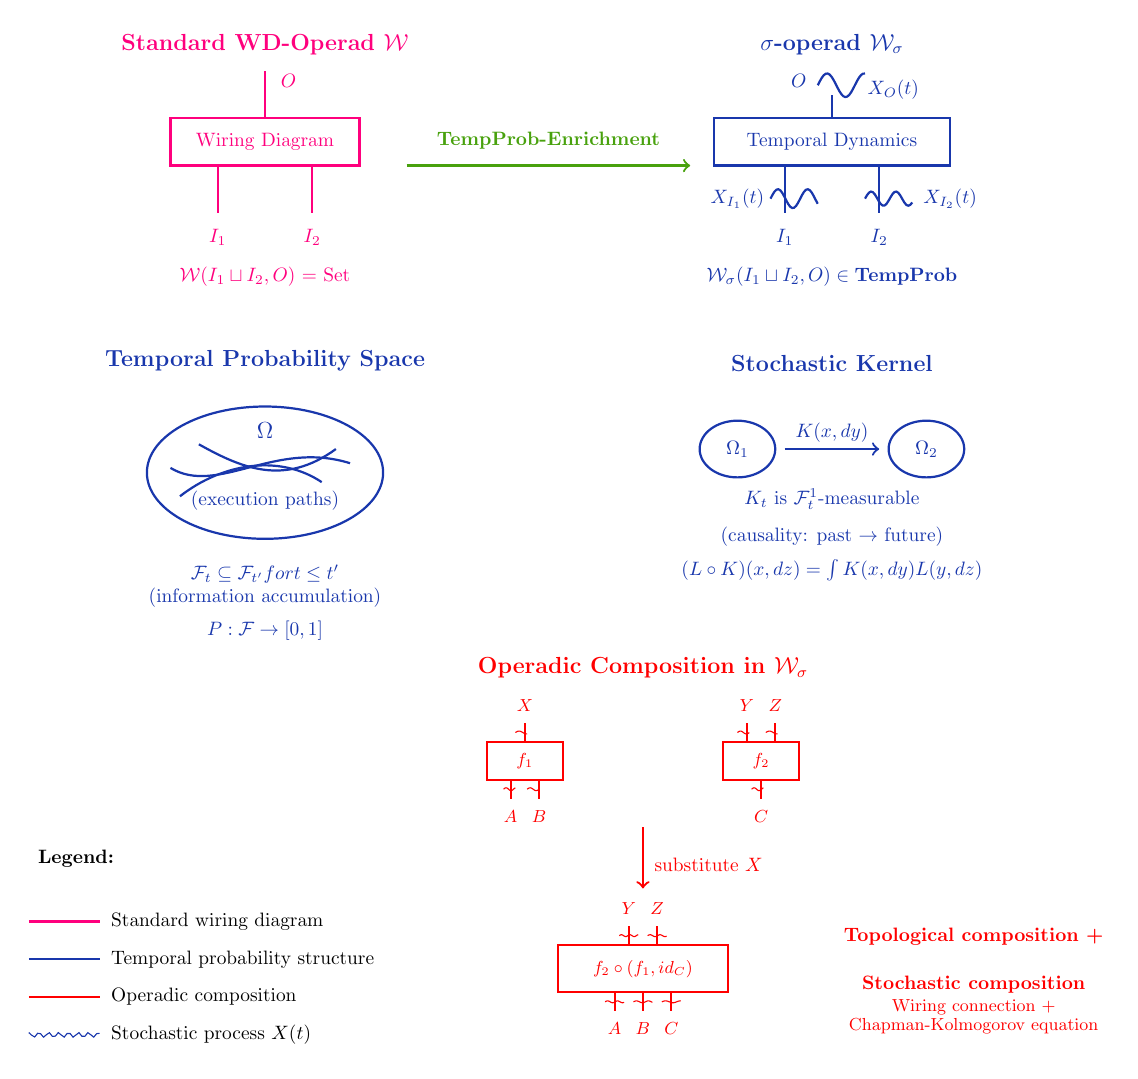
\begin{tikzpicture}[scale=0.6, every node/.style={scale=0.7}]

% Define colors - High Contrast Professional Palette
\definecolor{wdcolor}{RGB}{255, 0, 125}
\definecolor{tempcolor}{RGB}{25, 55, 172}
\definecolor{enrichcolor}{RGB}{72, 161, 13}
\definecolor{compcolor}{RGB}{255, 0, 0}

% Title
% \node[above] at (0, 8) {\Large\textbf{$\sigma$-operads: TempProb-Enriched Wiring Diagrams}};

% Part 1: Standard Wiring Diagram (left side)
\begin{scope}[shift={(-6, 4)}]
    \node[above, wdcolor, font=\large] at (0, 2.2) {\textbf{Standard WD-Operad $\mathcal{W}$}};

    % Input interfaces
    \draw[thick, wdcolor] (-1, -1) -- (-1, 0);
    \draw[thick, wdcolor] (1, -1) -- (1, 0);
    \node[below, wdcolor] at (-1, -1.2) {$I_1$};
    \node[below, wdcolor] at (1, -1.2) {$I_2$};

    % Box
    \draw[thick, wdcolor] (-2, 0) rectangle (2, 1);
    \node[wdcolor] at (0, 0.5) {Wiring Diagram};

    % Output interface
    \draw[thick, wdcolor] (0, 1) -- (0, 2);
    \node[above, wdcolor] at (0.5, 1.5) {$O$};

    % Hom-set notation
    \node[below, wdcolor] at (0, -2) {$\mathcal{W}(I_1 \sqcup I_2, O)$ = Set};
\end{scope}

% Arrow indicating enrichment
\draw[->, thick, enrichcolor] (-3, 4) -- (3, 4);
\node[above, enrichcolor] at (0, 4.2) {\textbf{TempProb-Enrichment}};

% Part 2: Temporal Probability Enriched (right side)
\begin{scope}[shift={(6, 4)}]
    \node[above, tempcolor, font=\large] at (0, 2.2) {\textbf{$\sigma$-operad $\mathcal{W}_\sigma$}};

    % Input interfaces with temporal processes
    \draw[thick, tempcolor] (-1, -1) -- (-1, 0);
    \draw[thick, tempcolor] (1, -1) -- (1, 0);
    \node[below, tempcolor] at (-1, -1.2) {$I_1$};
    \node[below, tempcolor] at (1, -1.2) {$I_2$};

    % Temporal processes at inputs
    \draw[tempcolor, thick, domain=0:1] plot (\x-1.3, {0.2*sin(10*\x r) - 0.7});
    \draw[tempcolor, thick, domain=0:1] plot (\x+0.7, {0.15*sin(12*\x r) - 0.7});
    \node[tempcolor] at (-2, -0.7) {$X_{I_1}(t)$};
    \node[tempcolor] at (2.5, -0.7) {$X_{I_2}(t)$};

    % Box with temporal dynamics
    \draw[thick, tempcolor] (-2.5, 0) rectangle (2.5, 1);
    \node[tempcolor] at (0, 0.5) {Temporal Dynamics};

    % Output with temporal process
    \draw[thick, tempcolor] (0, 1) -- (0, 1.5);
    \node[above, tempcolor] at (-0.7, 1.5) {$O$};
    \draw[tempcolor, thick, domain=0:1] plot (\x-0.3, {0.25*sin(8*\x r) + 1.7});
    \node[tempcolor] at (1.3, 1.6) {$X_O(t)$};

    % Hom-object notation
    \node[below, tempcolor] at (0, -2) {$\mathcal{W}_\sigma(I_1 \sqcup I_2, O) \in \mathbf{TempProb}$};
\end{scope}

% Part 3: Temporal Probability Space Details (middle-left)
\begin{scope}[shift={(-6, -2.5)}]
    \node[above, tempcolor, font=\large] at (0, 2) {\textbf{Temporal Probability Space}};

    % Sample space
    \draw[thick, tempcolor] (0, 0) ellipse (2.5 and 1.4);
    \node[tempcolor, font=\large] at (0, 0.9) {$\Omega$};
    \node[tempcolor] at (0, -0.6) {(execution paths)};

    % Trajectories
    \draw[tempcolor, thick] (-1.8, -0.5) .. controls (-0.9, 0.2) and (0.3, 0.4) .. (1.2, -0.2);
    \draw[tempcolor, thick] (-1.4, 0.6) .. controls (-0.5, 0.1) and (0.4, -0.3) .. (1.5, 0.5);
    \draw[tempcolor, thick] (-2.0, 0.1) .. controls (-1.0, -0.5) and (0.2, 0.7) .. (1.8, 0.2);

    % Filtration
    \node[below, tempcolor] at (0, -1.8) {$\mathcal{F}_t \subseteq \mathcal{F}_{t'} \text{ for } t \leq t'$};
    \node[below, tempcolor] at (0, -2.3) {(information accumulation)};

    % Measure
    \node[below, tempcolor] at (0, -3) {$\mathbb{P}: \mathcal{F} \to [0,1]$};
\end{scope}

% Part 4: Stochastic Kernel (middle-right)
\begin{scope}[shift={(6, -2.5)}]
    \node[above, tempcolor, font=\large] at (0, 2) {\textbf{Stochastic Kernel}};

    % Source space
    \draw[thick, tempcolor] (-2, 0.5) ellipse (0.8 and 0.6);
    \node[tempcolor] at (-2, 0.5) {$\Omega_1$};

    % Target space
    \draw[thick, tempcolor] (2, 0.5) ellipse (0.8 and 0.6);
    \node[tempcolor] at (2, 0.5) {$\Omega_2$};

    % Kernel arrow
    \draw[->, thick, tempcolor] (-1, 0.5) -- (1, 0.5);
    \node[above, tempcolor] at (0, 0.5) {$K(x, dy)$};

    % Adaptedness condition
    \node[below, tempcolor] at (0, -0.2) {$K_t$ is $\mathcal{F}_t^1$-measurable};
    \node[below, tempcolor] at (0, -1) {(causality: past $\to$ future)};

    % Chapman-Kolmogorov
    \node[below, tempcolor] at (0, -1.7) {$(L \circ K)(x, dz) = \int K(x, dy) L(y, dz)$};
\end{scope}

% Part 5: Composition Diagram (bottom)
\begin{scope}[shift={(2, -10)}]
    \node[above, compcolor, font=\large] at (0, 3) {\textbf{Operadic Composition in $\mathcal{W}_\sigma$}};

    % First component
    \begin{scope}[shift={(-2.5, 1)}]
        \draw[thick, compcolor] (-0.8, 0) rectangle (0.8, 0.8);
        \node[compcolor, font=\small] at (0, 0.4) {$f_1$};

        \draw[thick, compcolor] (-0.3, 0) -- (-0.3, -0.4);
        \draw[thick, compcolor] (0.3, 0) -- (0.3, -0.4);
        \node[below, compcolor, font=\small] at (-0.3, -0.5) {$A$};
        \node[below, compcolor, font=\small] at (0.3, -0.5) {$B$};

        \draw[thick, compcolor] (0, 0.8) -- (0, 1.2);
        \node[above, compcolor, font=\small] at (0, 1.3) {$X$};

        % Temporal processes (smaller)
        \draw[compcolor, domain=0:0.25] plot (\x-0.45, {0.03*sin(30*\x r) + -0.2});
        \draw[compcolor, domain=0:0.25] plot (\x+0.05, {0.03*sin(25*\x r) + -0.2});
        \draw[compcolor, domain=0:0.25] plot (\x-0.2, {0.03*sin(20*\x r) + 1.0});
    \end{scope}

    % Second component
    \begin{scope}[shift={(2.5, 1)}]
        \draw[thick, compcolor] (-0.8, 0) rectangle (0.8, 0.8);
        \node[compcolor, font=\small] at (0, 0.4) {$f_2$};

        \draw[thick, compcolor] (0, 0) -- (0, -0.4);
        \node[below, compcolor, font=\small] at (0, -0.5) {$C$};

        \draw[thick, compcolor] (-0.3, 0.8) -- (-0.3, 1.2);
        \draw[thick, compcolor] (0.3, 0.8) -- (0.3, 1.2);
        \node[above, compcolor, font=\small] at (-0.3, 1.3) {$Y$};
        \node[above, compcolor, font=\small] at (0.3, 1.3) {$Z$};

        % Temporal processes (smaller)
        \draw[compcolor, domain=0:0.25] plot (\x-0.2, {0.03*sin(30*\x r) + -0.2});
        \draw[compcolor, domain=0:0.25] plot (\x-0.5, {0.03*sin(25*\x r) + 1.0});
        \draw[compcolor, domain=0:0.25] plot (\x+0.1, {0.03*sin(20*\x r) + 1.0});
    \end{scope}

    % Composition arrow (Vertical now)
    \draw[->, thick, compcolor] (0, 0) -- (0, -1.3);
    \node[right, compcolor] at (0.1, -0.8) {substitute $X$};

    % Composed system
    \begin{scope}[shift={(0, -3.5)}]
        \draw[thick, compcolor] (-1.8, 0) rectangle (1.8, 1);
        \node[compcolor, font=\small] at (0, 0.5) {$f_2 \circ (f_1, \text{id}_C)$};

        % Inputs
        \draw[thick, compcolor] (-0.6, 0) -- (-0.6, -0.4);
        \draw[thick, compcolor] (0, 0) -- (0, -0.4);
        \draw[thick, compcolor] (0.6, 0) -- (0.6, -0.4);
        \node[below, compcolor, font=\small] at (-0.6, -0.5) {$A$};
        \node[below, compcolor, font=\small] at (0, -0.5) {$B$};
        \node[below, compcolor, font=\small] at (0.6, -0.5) {$C$};

        % Outputs
        \draw[thick, compcolor] (-0.3, 1) -- (-0.3, 1.4);
        \draw[thick, compcolor] (0.3, 1) -- (0.3, 1.4);
        \node[above, compcolor, font=\small] at (-0.3, 1.5) {$Y$};
        \node[above, compcolor, font=\small] at (0.3, 1.5) {$Z$};

        % Temporal processes (smaller and better positioned)
        \draw[compcolor, domain=0:0.4] plot (\x-0.8, {0.02*sin(30*\x r) + -0.2});
        \draw[compcolor, domain=0:0.4] plot (\x-0.2, {0.02*sin(25*\x r) + -0.2});
        \draw[compcolor, domain=0:0.4] plot (\x+0.4, {0.02*sin(20*\x r) + -0.2});
        \draw[compcolor, domain=0:0.4] plot (\x-0.5, {0.02*sin(35*\x r) + 1.2});
        \draw[compcolor, domain=0:0.4] plot (\x+0.1, {0.02*sin(30*\x r) + 1.2});
    \end{scope}

    % Explanation
    \node[below, compcolor] at (7, -2) {\textbf{Topological composition +}};
    \node[below, compcolor] at (7, -3) {\textbf{Stochastic composition}};
    \node[below, compcolor, font=\small] at (7, -3.5) {Wiring connection +};
    \node[below, compcolor, font=\small] at (7, -3.9) {Chapman-Kolmogorov equation};
\end{scope}

% Legend
\begin{scope}[shift={(-10, -12)}]
    \node[above] at (0, 1) {\textbf{Legend:}};

    \draw[thick, wdcolor] (-1, 0) -- (0.5, 0);
    \node[right] at (0.6, 0) {Standard wiring diagram};

    \draw[thick, tempcolor] (-1, -0.8) -- (0.5, -0.8);
    \node[right] at (0.6, -0.8) {Temporal probability structure};

    \draw[thick, compcolor] (-1, -1.6) -- (0.5, -1.6);
    \node[right] at (0.6, -1.6) {Operadic composition};

    \draw[tempcolor, domain=-1:0.5] plot (\x, {0.05*sin(30*\x r) + -2.4});
    \node[right] at (0.6, -2.4) {Stochastic process $X(t)$};
\end{scope}

\end{tikzpicture}

\caption{$\sigma$-operads as TempProb-enriched wiring diagrams. The top shows the enrichment process: standard wiring diagrams (left) become enriched with temporal probability structures (right), where each port carries stochastic processes $X(t)$ and hom-objects are temporal probability spaces. The middle illustrates the components: temporal probability spaces with filtrations and stochastic kernels preserving causality. The bottom demonstrates operadic composition, combining topological wiring with stochastic composition via the Chapman-Kolmogorov equation.}
\label{fig:sigma_operad}
\end{figure}

\subsubsection{Temporal Causality through Ports}

In $\sigma$-operads, each port carries temporal probabilistic information:
\begin{itemize}
    \item Each port $p$ is associated with an adapted stochastic process $X_p = \{X_p(t)\}_{t \geq 0}$ representing the temporal evolution of information at that interface.
    \item Wires connecting ports encode conditional temporal dependence: if port $p$ connects to port $q$, then $X_q(t)$ depends on the history $\{X_p(s)\}_{s \leq t}$. For the markovian case, this dependence is only on $X_p(t)$.
    \item The filtration structure ensures causality: information flows from past to future, never backwards in time, so even though $\Omega$ contains all trajectories, the filteration removes (or assigns zero probability to) any trajectories that violate causal ordering.
\end{itemize}

\subsubsection{Composition of Temporal Morphisms}

When composing morphisms in $\mathcal{W}_{\sigma}$, we combine both the topological composition of wiring diagrams and the stochastic composition in $\mathbf{TempProb}$:

\begin{enumerate}
    \item \textbf{Topological Composition}: Standard wiring diagram composition connects outputs to inputs through interface matching. The resulting wiring diagram represents the overall system architecture with overall inputs and outputs.
    \item \textbf{Temporal Composition}: The stochastic processes at connected ports are composed using the Chapman-Kolmogorov equation, ensuring that temporal dependencies chain correctly through the composite system.
    \item \textbf{Filtration Compatibility}: The composed system's filtration is the natural extension that preserves the temporal ordering and causal structure. This prevents two operads from "looking into the future" of one another during composition.
\end{enumerate}

This composition naturally models how complex systems evolve: subsystems with their own temporal dynamics are connected through their interfaces, creating a larger system whose temporal evolution respects the causal flow through the network structure.
